\section{Method}
\label{sec:method}
\begin{table}[H]
  \centering
  \newcolumntype{Y}{>{\centering\arraybackslash}X}
  \begin{tabularx}{\linewidth}{Y X}
    \Xhline{1pt}
    Abridge & Full Name \\
    \Xhline{1pt}
    ADC & Analog-to-Digital Conversion \\
    IDE & Integrated Development Environment \\
    \Xhline{1pt}
  \end{tabularx}
  \label{tab:table}
\end{table}
\textbf{Keywords}: ``distance-angle'' radar chart, ADC, control variable, Ultrasonic distance measurement

\subsection*{Experient: Measurement of the maximum distance that can be measured to an obstacle at different angles}
To achieve the function, we have carefully designed the following circuit diagram (Figure~\ref{fig:circuit-diagram}):

\begin{figure}[H]
  \centering
  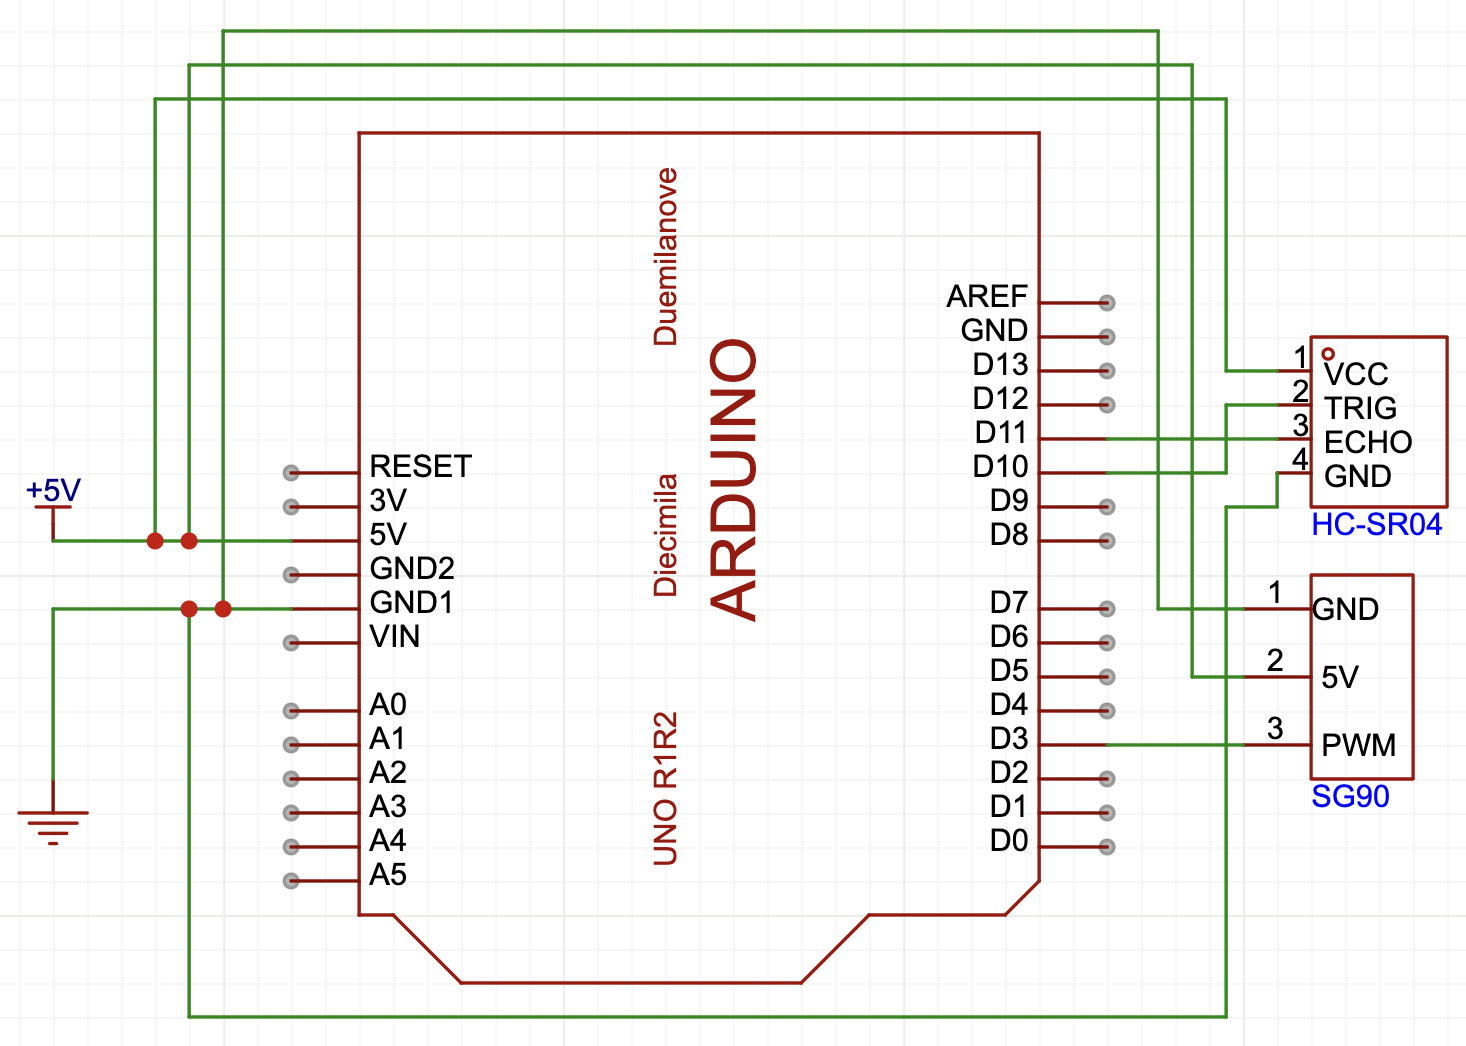
\includegraphics[width=0.6\linewidth]{../Photos/jlc/jlc}
  \rule{35em}{0.5pt}
  \caption{circuit diagram}
  \label{fig:circuit-diagram}
\end{figure}

In accordance with the designed circuit diagram,
the actual wiring (Figure~\ref{fig:actual-wiring}) of our vehicle (front and above) is as follows:

\begin{figure}[H]
  \centering
  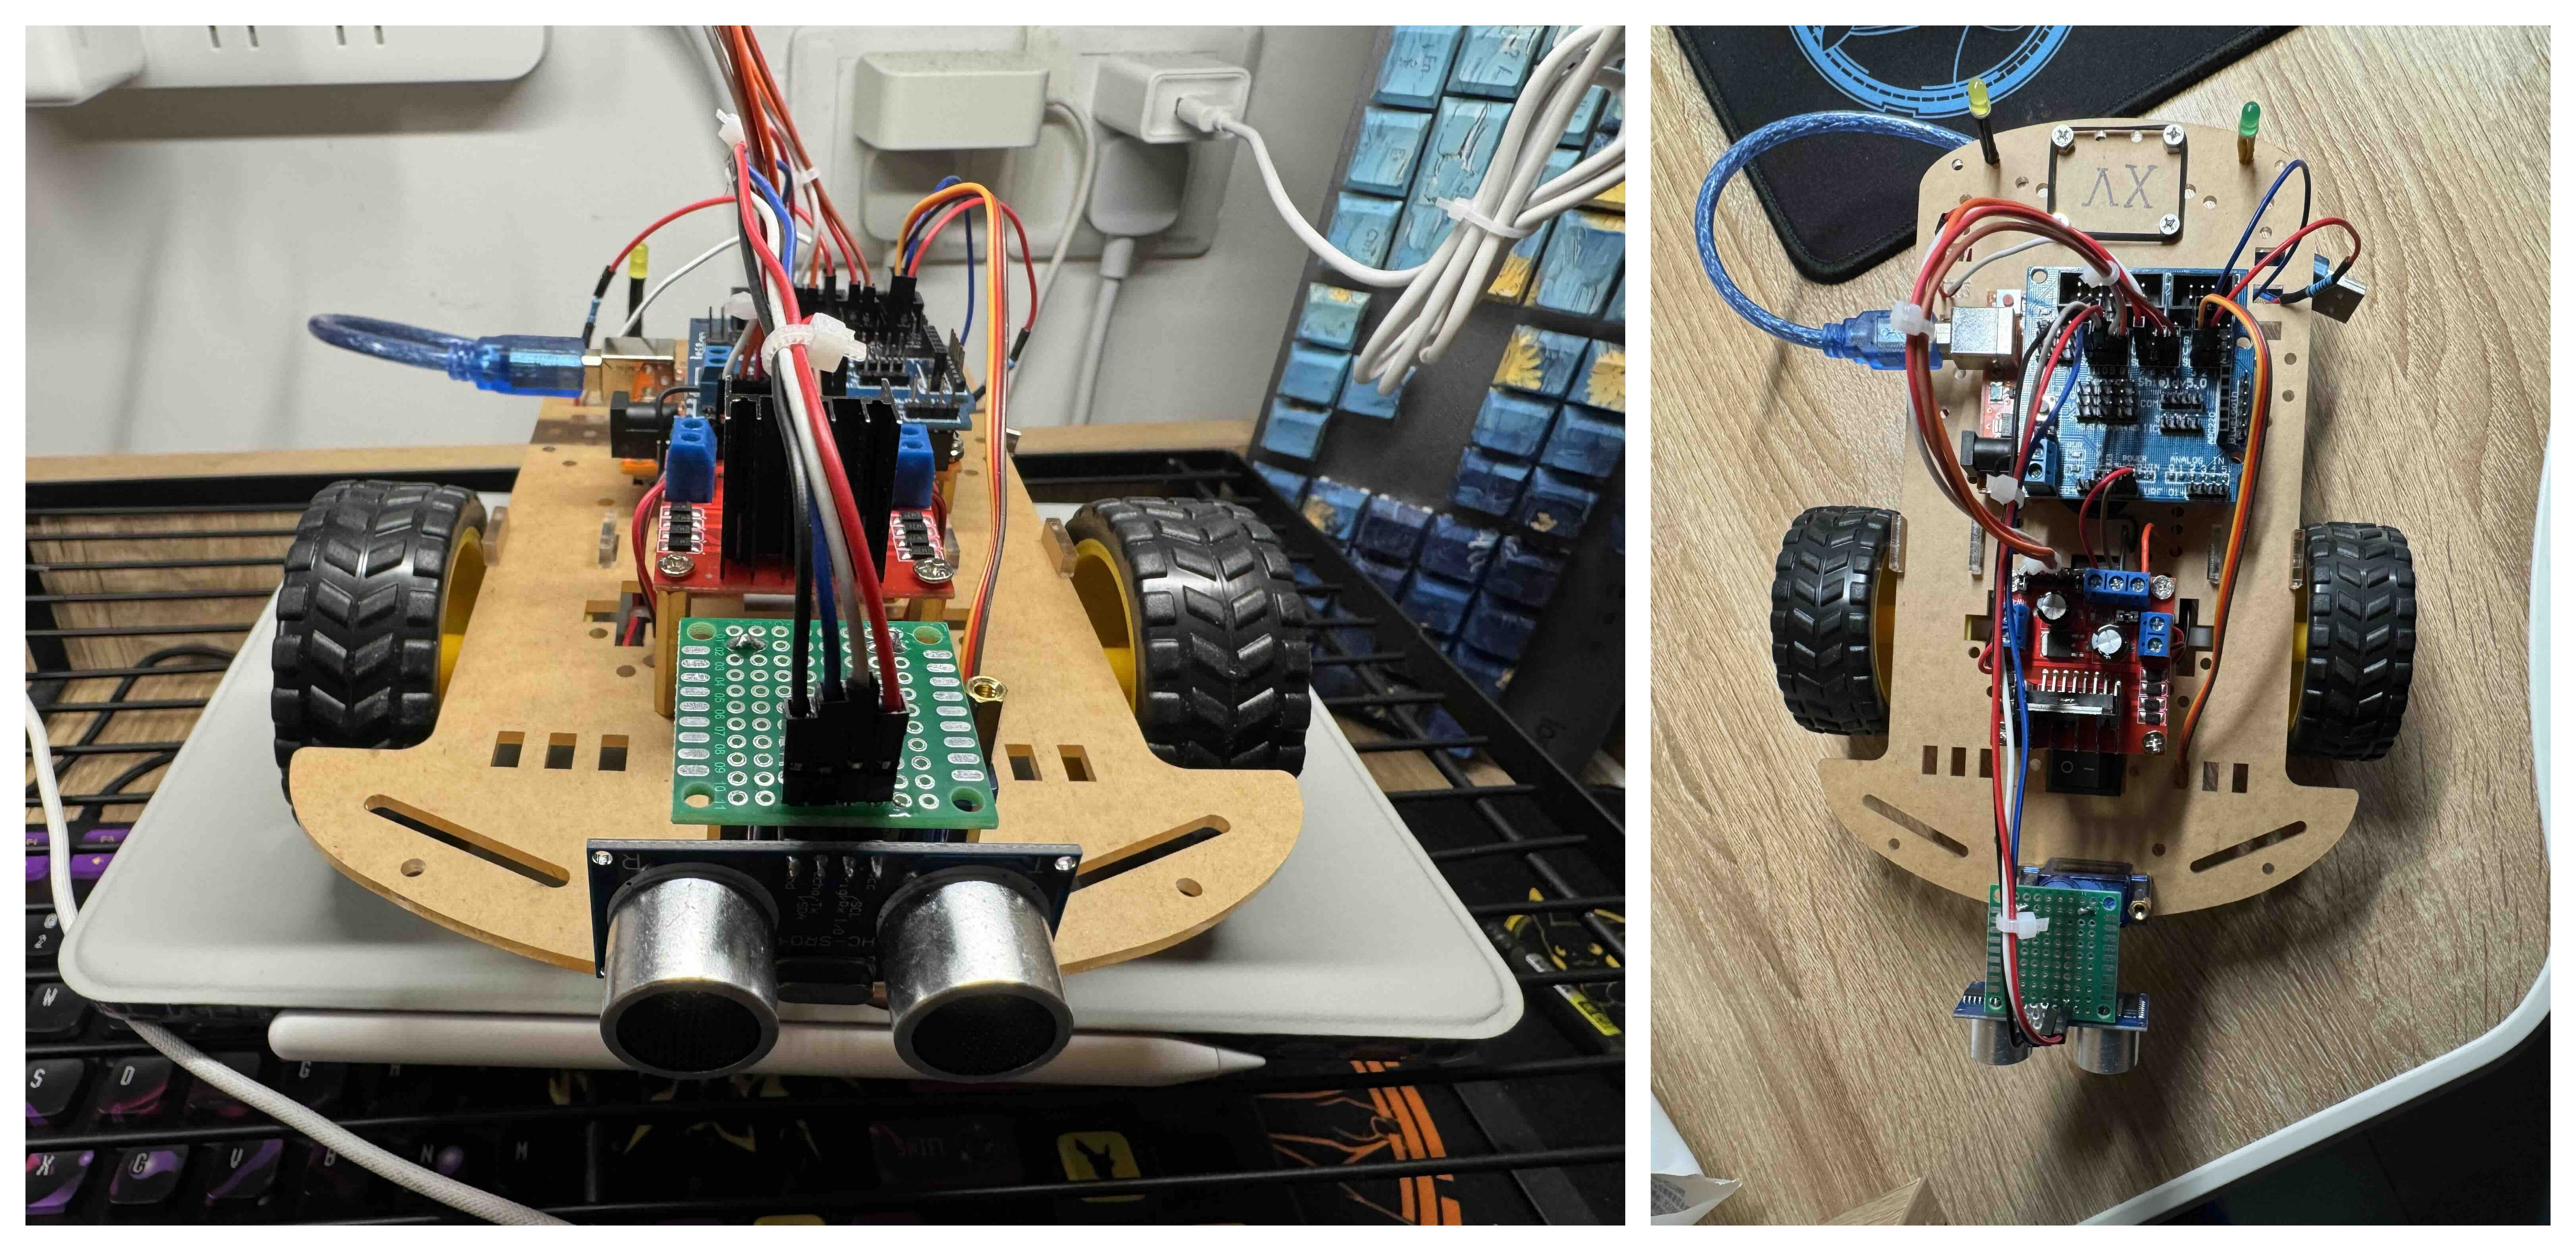
\includegraphics[width=0.8\linewidth]{Figures/actual-wiring}
  \rule{35em}{0.5pt}
  \caption{actual wiring of vehicle}
  \label{fig:actual-wiring}
\end{figure}

After selecting the obstacle, measurements are taken at intervals of 40 centimeters within a range of 0 to 400 centimeters from the obstacle.
The measurement angles span from 0 to 180 degrees, with the direction directly in front of the vehicle's nose defined as 90 degrees.
The formulas~\ref{eq:distance} used are as follows:

\begin{equation}
  Distance = Velocity \times Time
  \label{eq:distance}
\end{equation}

In the experimental environment, where the air is dry and the temperature is 20 degrees Celsius,
the speed of sound is approximately 343 meters per second, which is equivalent to 34,300 centimeters per second.
Since the ultrasonic wave travels twice the distance from the transmitter to the target and back to the receiver,
the actual distance measurement is related to the time difference as follows:
a distance of 1 centimeter corresponds to a time difference of 58.3 microseconds, which
can be approximated to 58 microseconds for simplified calculations.
